\section{Online Deployment and Performance}%
\label{sec:operation}


 During to 2017-2018 years in Run 2, the actual \rnn{} implementation can be partitioned into four chronological stages:

\begin{enumerate}[i]
  \item A development stage up to early 2017, where the \rnn{}
      potential was estimated from trigger emulation and data reprocessing;
  \item The commissioning stage (\SI{5.4}{\per\femto\barn}) occurred in
      early 2017 runs, where all primary
      triggers were duplicated with either the \rnn{} or cut-based algorithms
      operating in the \fastcalo{} stage of the HLT;
  \item The operation of the method as the baseline trigger, which occurred after 2017 Technical Stop 1 (TS1). For
    monitoring purposes, and to allow precise statistical evaluation of eventual
    disagreements between the \fastcalo{} methods from an offline
    perspective (Section~\ref{sec:off_ana}), a duplicated trigger pair, i.e.
    with and without \rnn{}, was kept operating unprescaled during this period
    (\SI{39.0}{\per\femto\barn}). Here, the efficiencies of the
    duplicated triggers in 2017 (Section~\ref{ssec:2017_ringer_operation}) are compared;
  \item Finally, the duplicated trigger was removed for 2018 operation.
    Therefore, the evaluation of 2018 \rnn{} operation relying on a comparison with
    2017 efficiency is presented in Section~\ref{ssec:2018_ringer_operation}.
\end{enumerate}

This section reports the \rnn{} operation in each one of these periods. Additionally, the discussion about CPU time will be covered in Section~\ref{ssec:cpu_reduction}.

\subsection{2017 Operation}\label{ssec:2017_ringer_operation}

A backup single electron HLT\_e28\_lhtight\_nod0\_(noringer)\_ivarloose trigger
 with and without (noringer) the \rnn{} was employed for monitoring purposes after the first technical stop (TS1).
This trigger require an electron candidate with $E_T > 28$ GeV satisfying the tight selection (lhtight\_nod0) with a loosest isolation criteria (ivarloose). During the monitoring process, a similar operation of both triggers was observed in terms of signal efficiency using the integrated luminosity along the period, as shown in Figure~\ref{fig:2017_zee_triggers} left side. The trigger
turn-on curves exhibit similar profile. In $\eta$, the \rnn{} shows a reasonably symmetric profile with respect to positive and negative $\eta$. In addition, a difference of about half to one percentage point may be observed in $\eta$ because of the transition region between the endcap and barrel. Besides aforementioned points, overall efficiency fluctuations are smaller than a few per-mille. Although a slightly more prominent efficiency loss with respect to
\avgmu{} is observed in Figure~\ref{fig:e28_comp_mu} for the \rnn{} trigger, the electron efficiency was kept nearly the same. Such loss occurs after the linear threshold correction limit of $\avgmu=40$ that was employed during 2017.

Other important triggers were assessed by comparing the trigger efficiencies on 2017 collision data collected before and after switching to the \rnn{} algorithms can be observed in Figure~\ref{fig:2017_zee_triggers} right side. The single electron HLT\_e17\_lhvloose\_nod0\_L1EM15VHI trigger require an electron candidate seeded by the Level-1 trigger L1\_EM15VHI with $E_T > 17$ GeV satisfying the loosest identification criteria (lhvloose). On the other hand, HLT\_e26\_lhtight\_nod0\_ivarloose and HLT\_e60\_lhmedium\_nod0 requires an electron candidate with $E_T>26$ Gev satisfying the tight identification (lhtight) with loosest isolation (ivarloose), and $E_T>60$ GeV satisfying the medium identification (lhmedium), respectively. Here, the electron efficiency was also kept nearly unchanged for relevant single electron triggers. Note that results in
this plot are computed with two different data taking periods: with or without the \rnn{} algorithm. 




\begin{figure}[h!tb]
  
  \begin{subfigure}[c]{.49\textwidth}
  \centering
  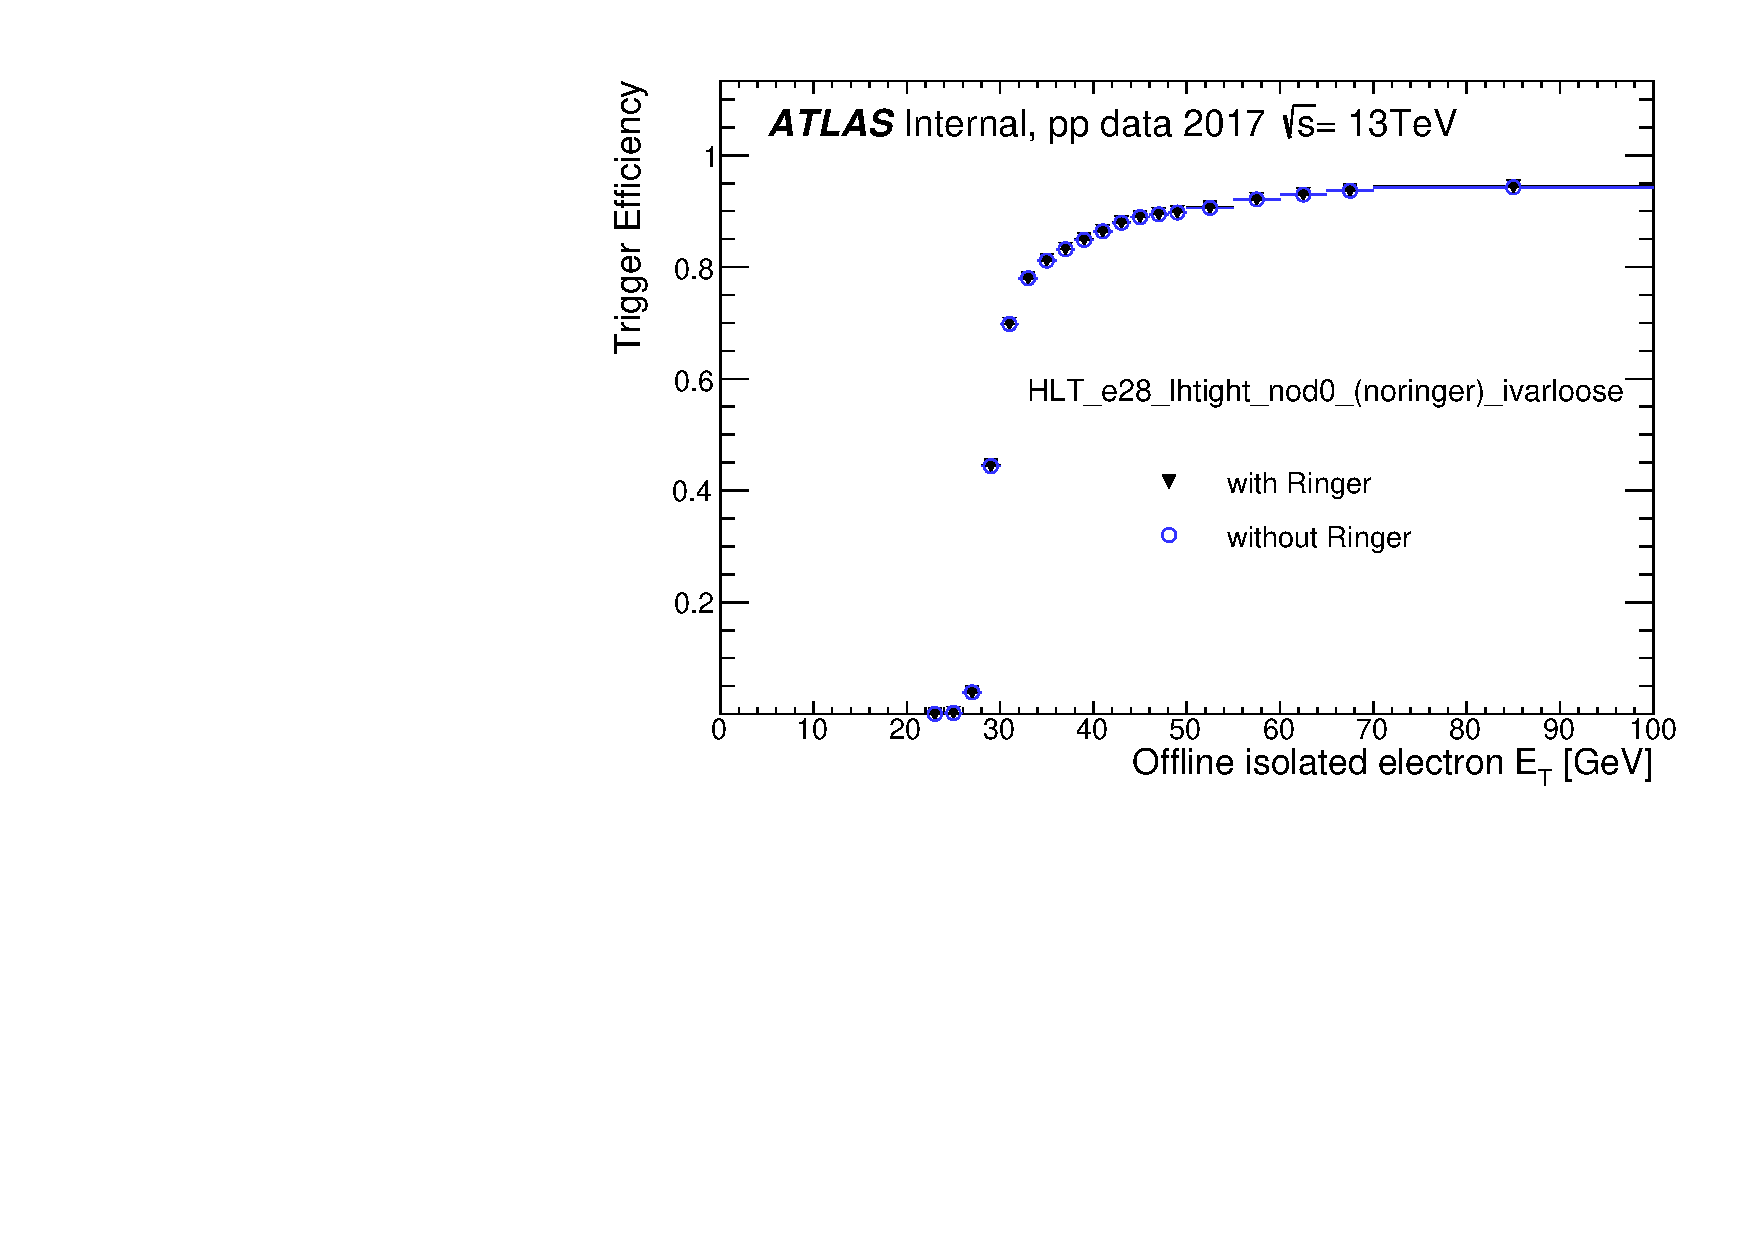
\includegraphics[width=\textwidth]{sections/03_operation/figures/efficiencies/eff_EGAM1_e28_ringer_and_noringer_2017_after_ts1_HLT_et.pdf}
  \caption{}
  \end{subfigure}
  %
  \begin{subfigure}[c]{.49\textwidth}
  \centering
  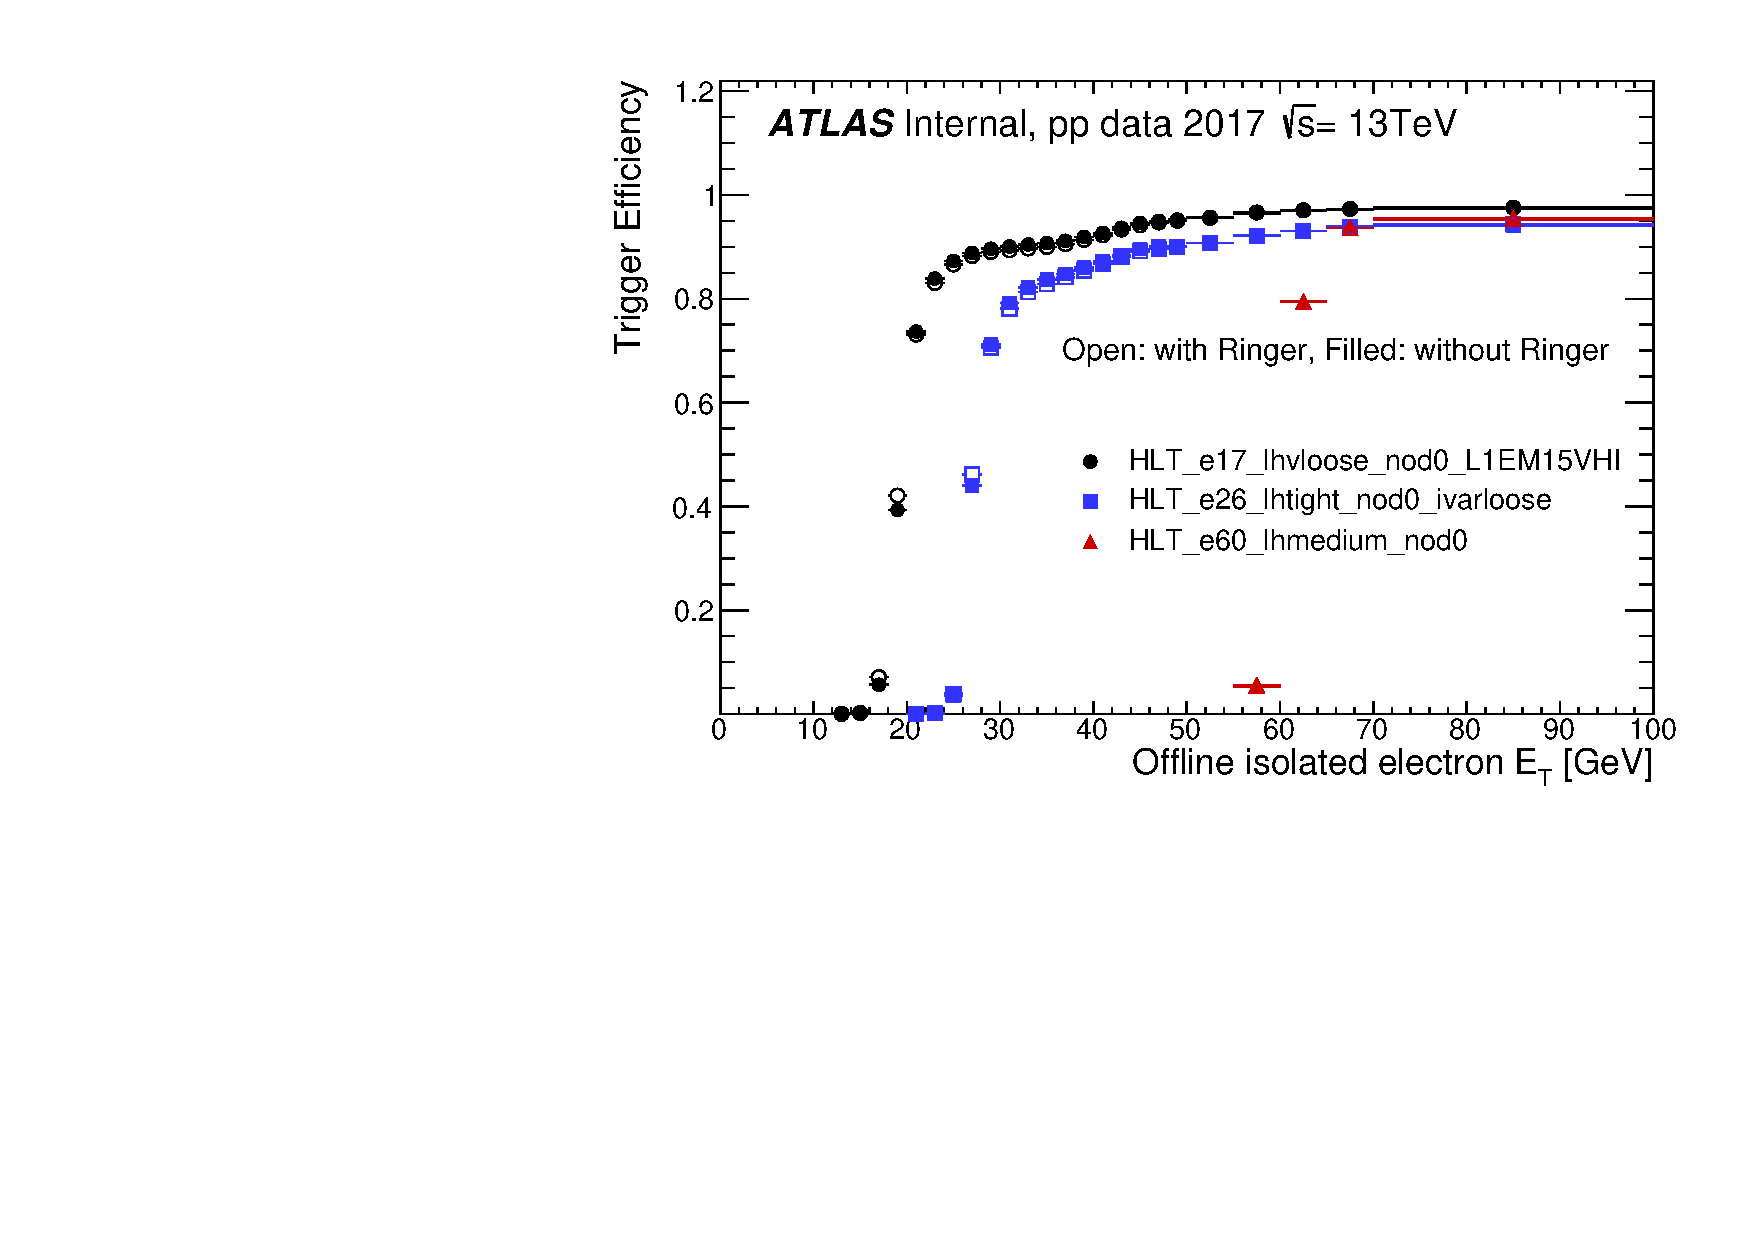
\includegraphics[width=\textwidth]{sections/03_operation/figures/efficiencies/eff_EGAM1_e17_e26_e60_2017_before_and_after_ts1_et.pdf}
  \caption{}%
  \end{subfigure}\\
  %
  \begin{subfigure}[c]{.49\textwidth}
  \centering
  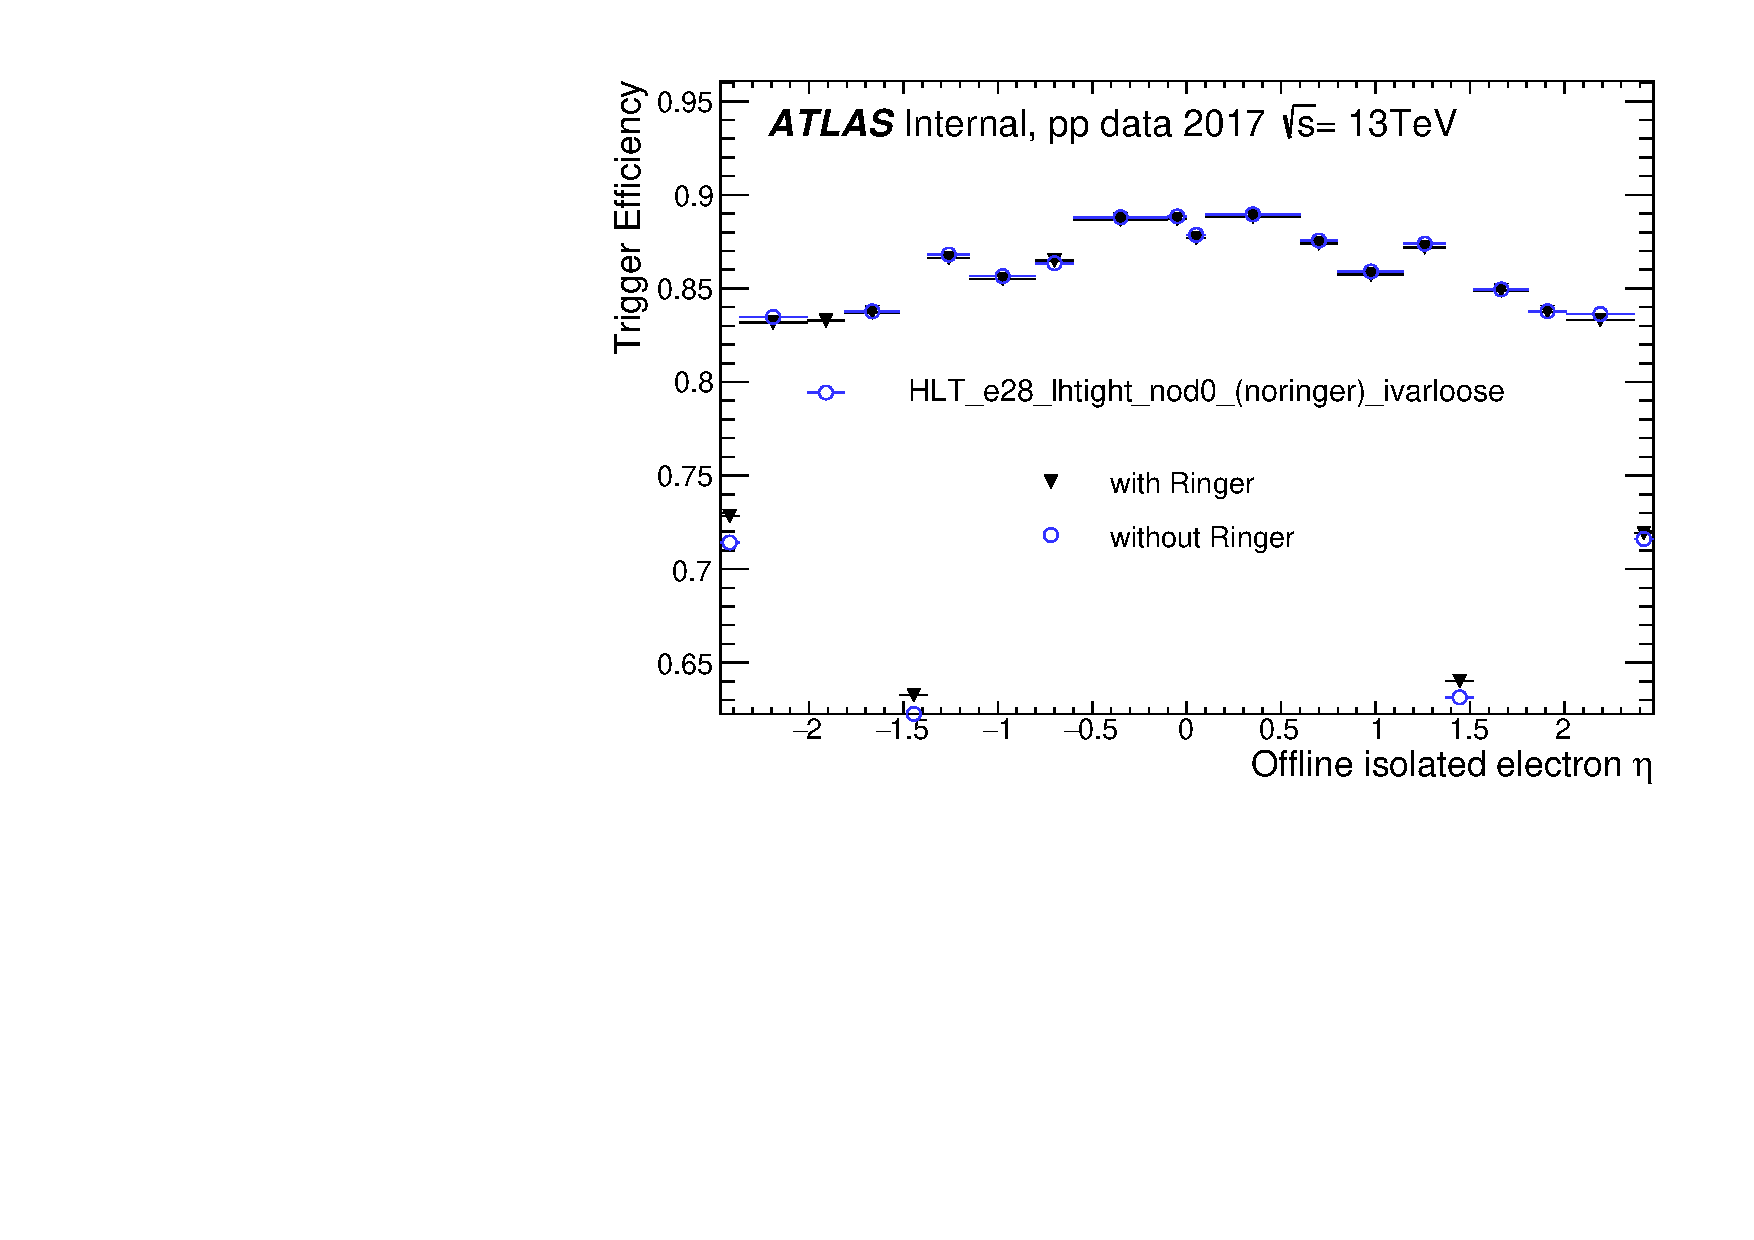
\includegraphics[width=\textwidth]{sections/03_operation/figures/efficiencies/eff_EGAM1_e28_ringer_and_noringer_2017_after_ts1_HLT_eta.pdf}
  \caption{}
  \end{subfigure}
  %
  \begin{subfigure}[c]{.49\textwidth}
  \centering
  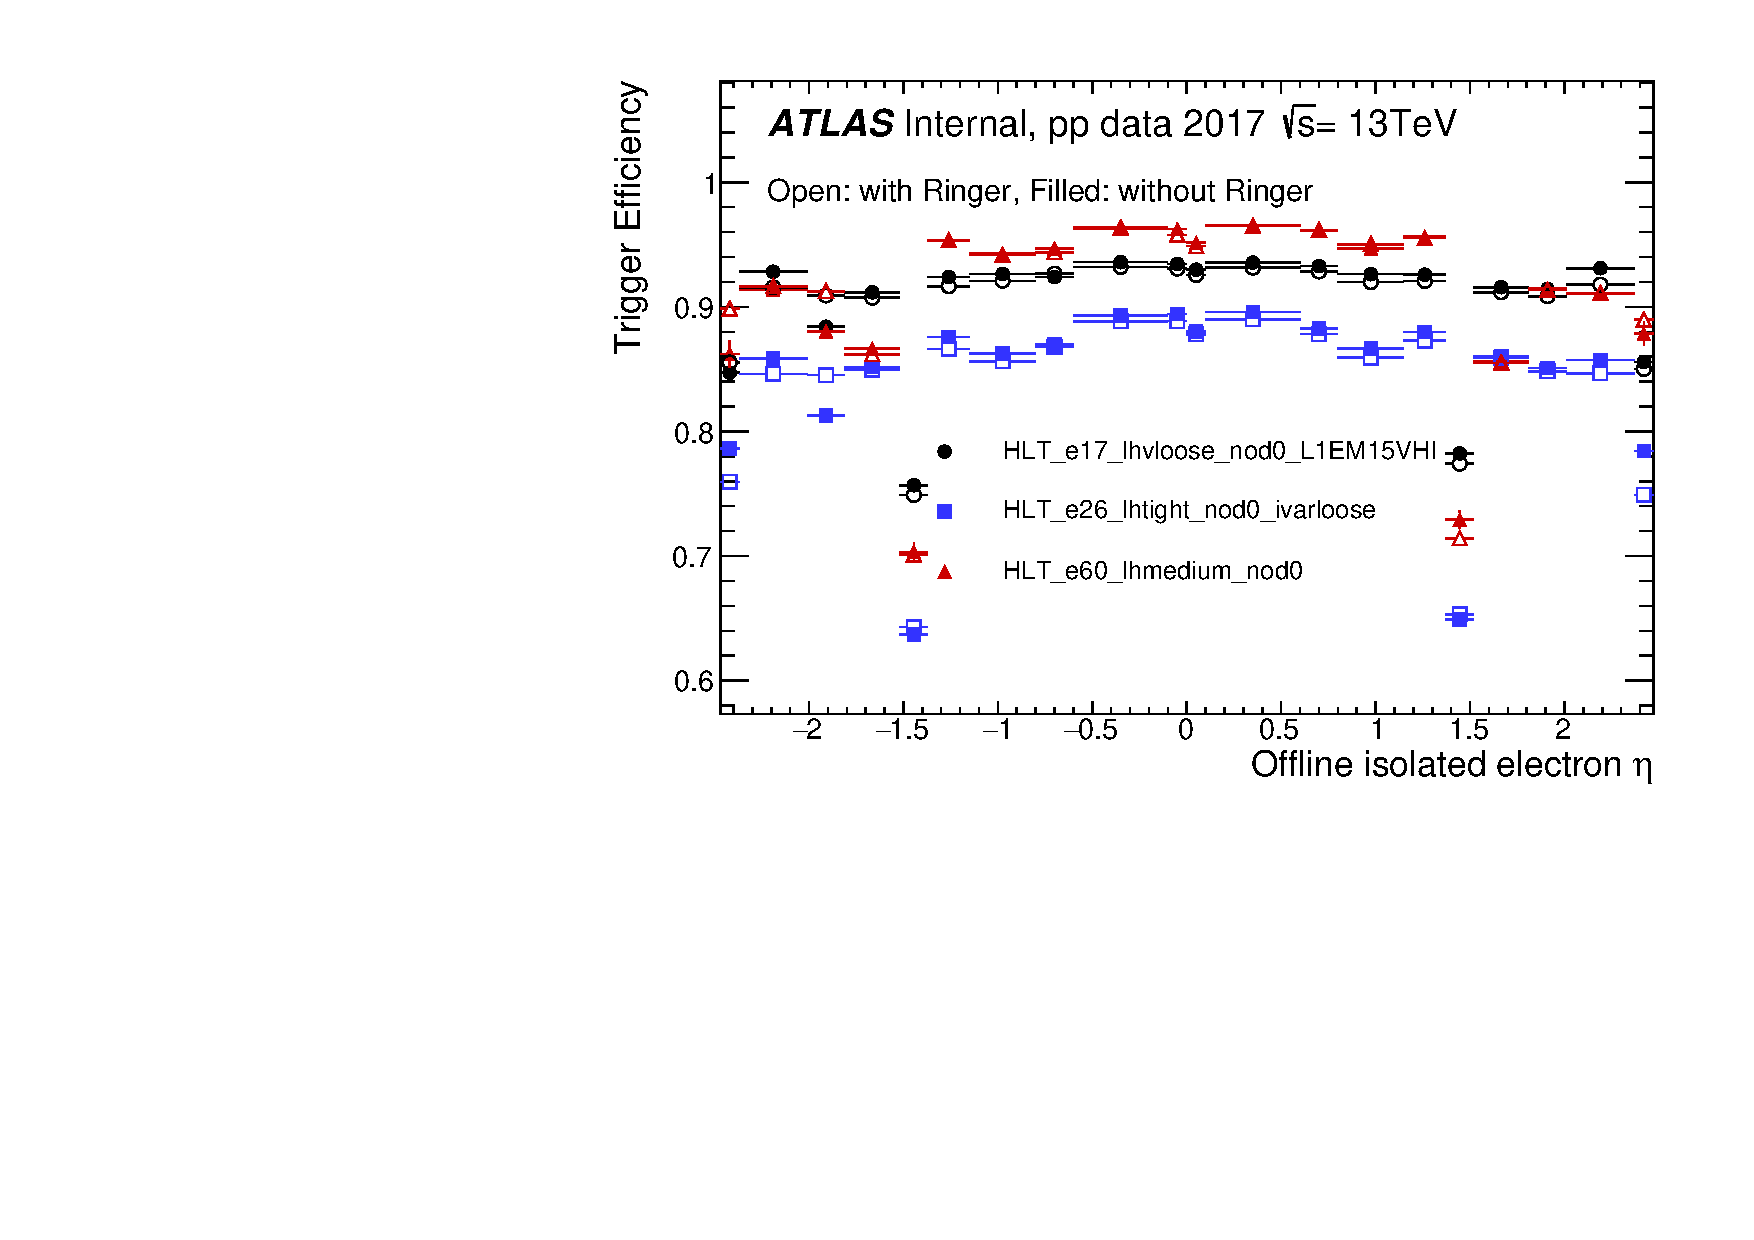
\includegraphics[width=\textwidth]{sections/03_operation/figures/efficiencies/eff_EGAM1_e17_e26_e60_2017_before_and_after_ts1_eta.pdf}
  \caption{}%
  \end{subfigure} \\
  %
  \begin{subfigure}[c]{.49\textwidth}
  \centering
  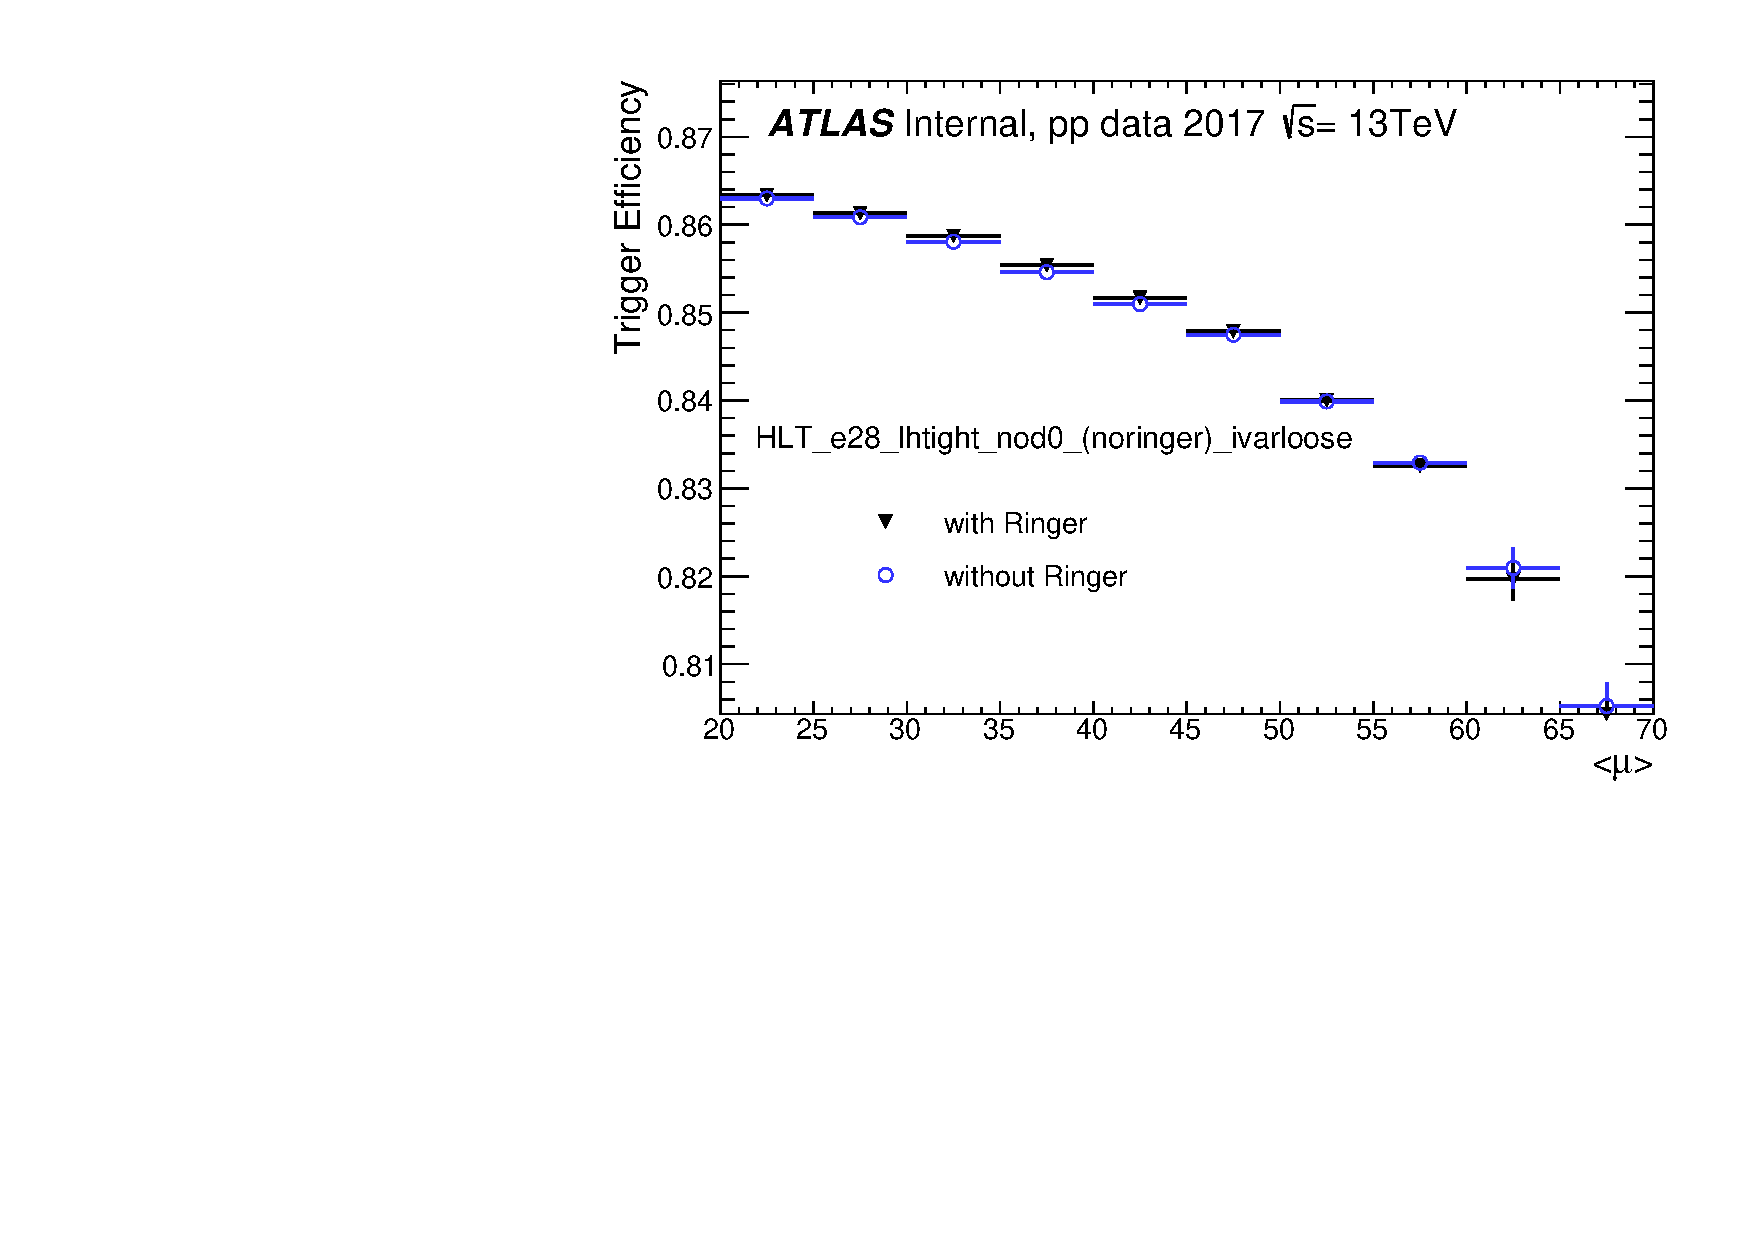
\includegraphics[width=\textwidth]{sections/03_operation/figures/efficiencies/eff_EGAM1_e28_ringer_and_noringer_2017_after_ts1_HLT_mu.pdf}
  \caption{}%
  \label{fig:e28_comp_mu}
  \end{subfigure}
  %
  \begin{subfigure}[c]{.49\textwidth}
  \centering
  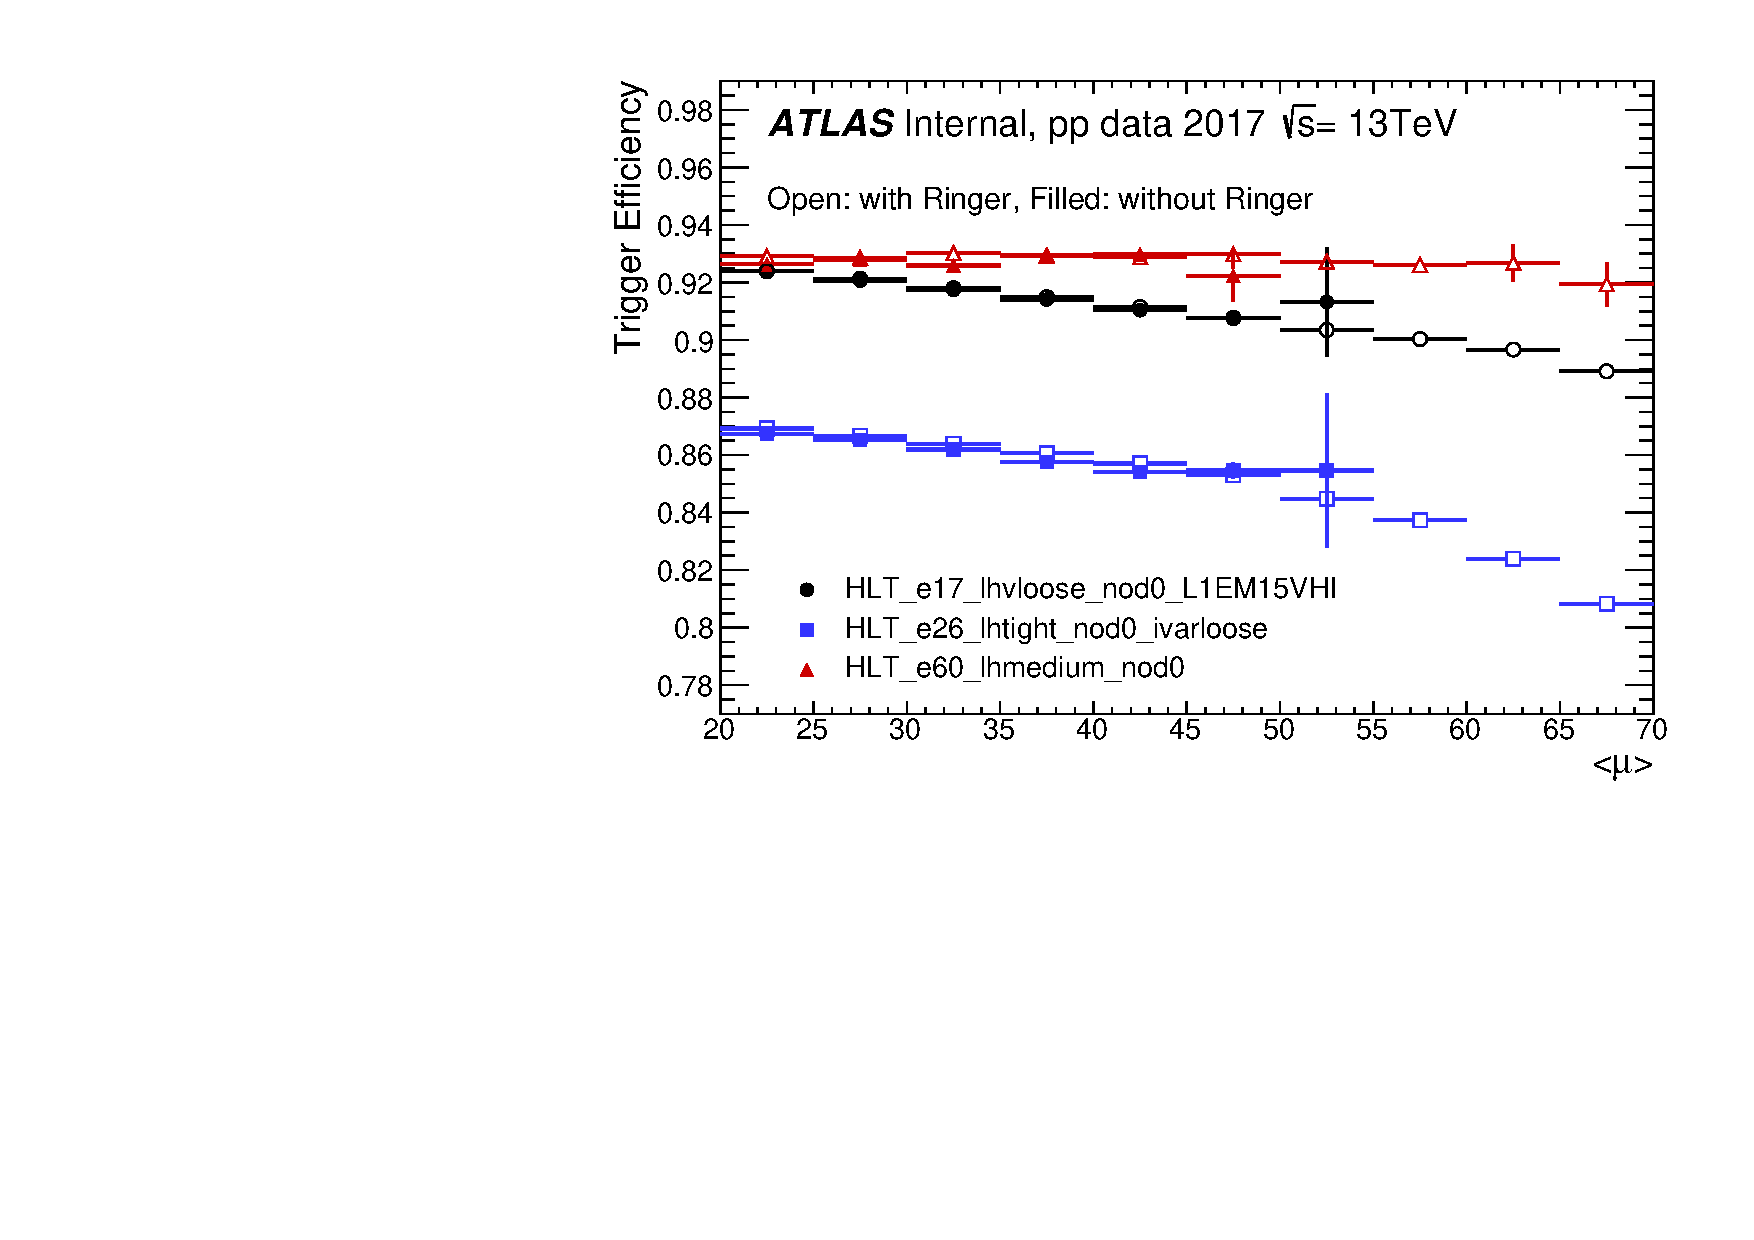
\includegraphics[width=\textwidth]{sections/03_operation/figures/efficiencies/eff_EGAM1_e17_e26_e60_2017_before_and_after_ts1_mu.pdf}
  \caption{}%
  \end{subfigure}
  
  \caption{Left: HLT electron efficiency as a function of \et{} (a), \eta{} (c) and \avgmu{} (e) for the single electron isolated trigger requiring $\et{} > \SI{28}{\GeV}$ and \tight{} selection with and without the \rnn{} algorithm employing 2017 collision data. Right: Efficiency of three single electron triggers as a function of \et (b), \eta (d) and \avgmu (f) for 2017 collision data. Open (closed) markers contain the efficiency measurements on runs before (after) the deployment of the \rnn{}, thus referring to triggers being executed without (with) the \rnn{} algorithm. For 2017 collision data, the higher \avgmu{} values were reached only after the deployment.}
  \label{fig:2017_zee_triggers}
\end{figure}




By contrasting the behavior of the duplicated trigger using fake electron collision data, it becomes clear the power of the \rnn{} algorithm. An overall reduction factor of
the fake rate by a factor of 13.75 is achieved at \fastcalo step. It can be seen in Figure~\ref{fig:2017_fake_triggers} left size, that the improvement at \fastcalo is similar for all
regions in the evaluated variables, particularly interesting when
considering the low \et{} and the end-cap regions. Besides the capability of improving early fake rejection, the usage of the \rnn{} also contributed to reduce the final fake rate at HLT step
(Figure~\ref{fig:2017_fake_triggers} right size) by a factor of 2, mostly coming from the transition regions in the calorimeter.



\begin{figure}[h!tb]
  \begin{subfigure}[c]{.49\textwidth}
  \centering
  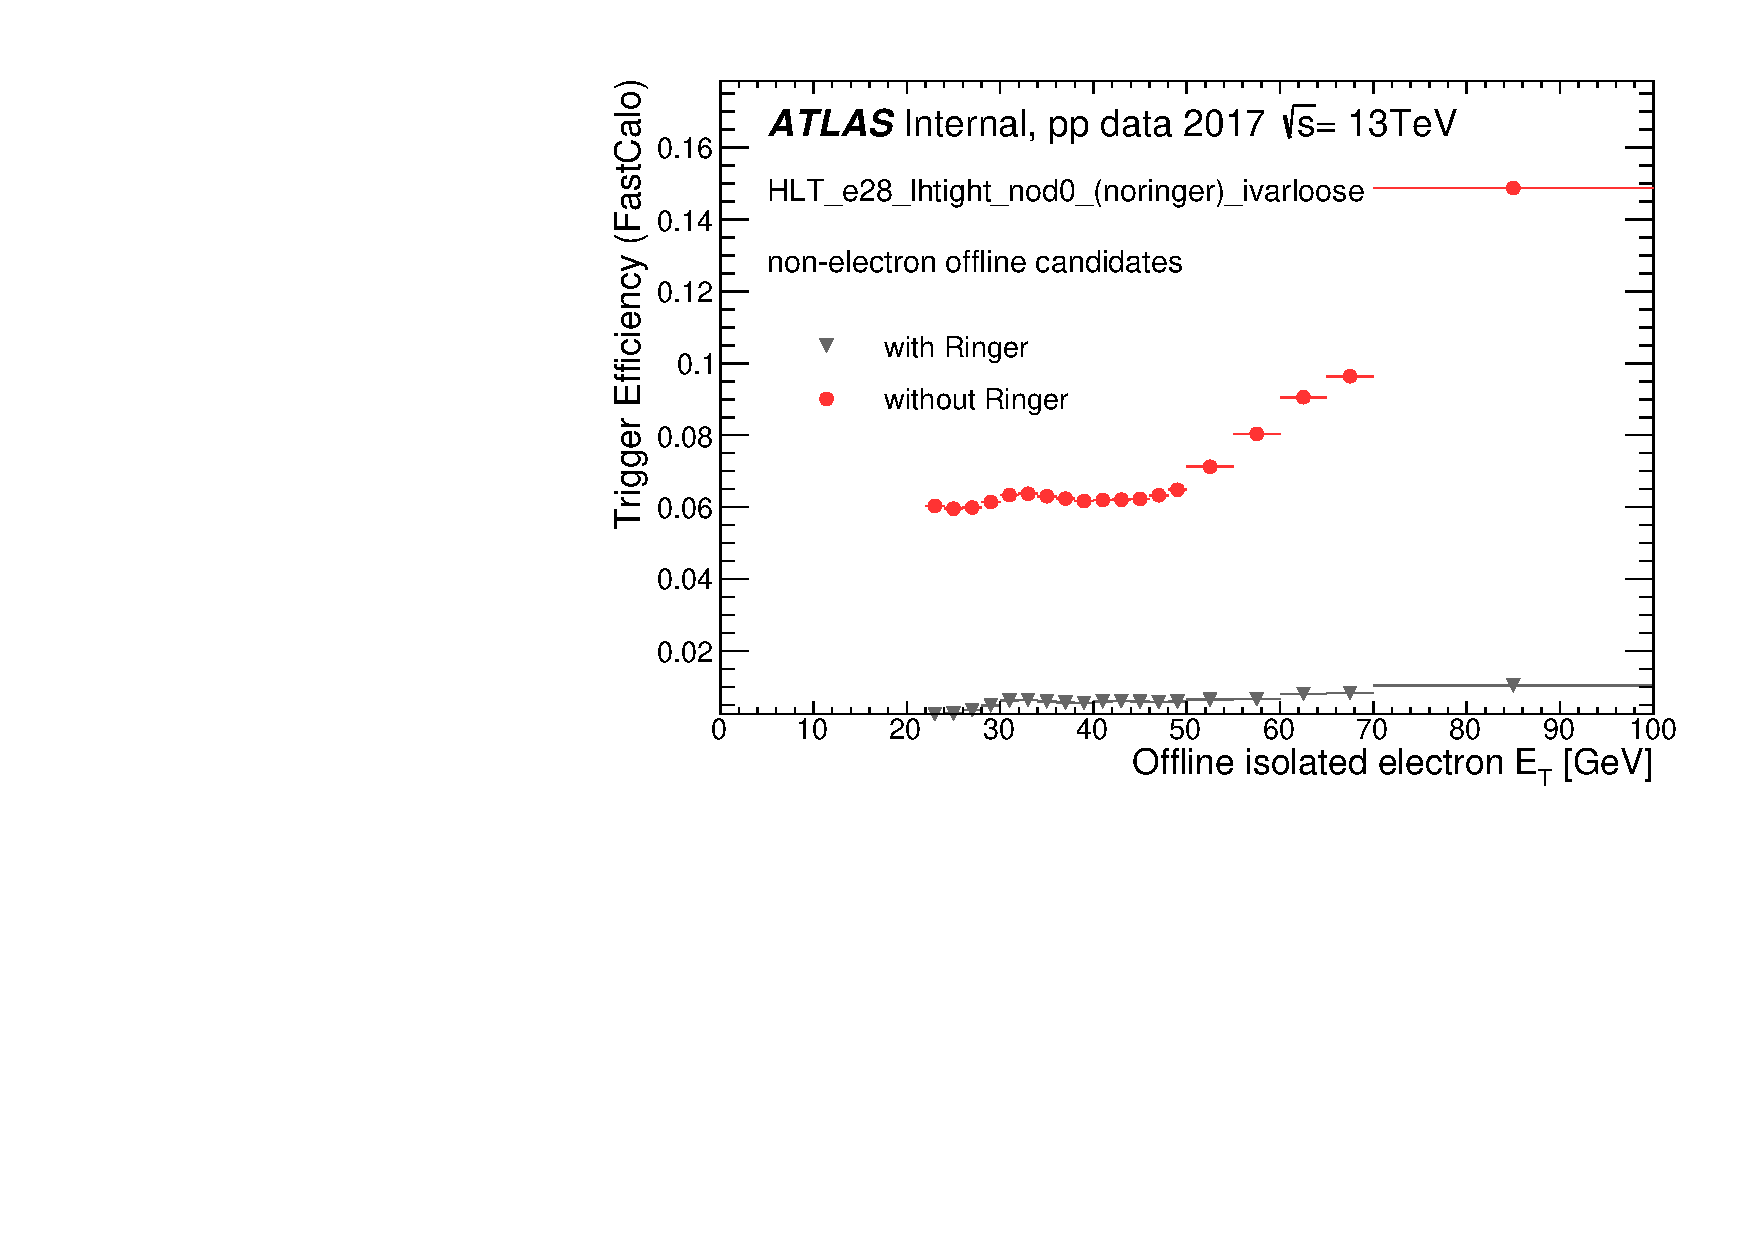
\includegraphics[width=\textwidth]{sections/03_operation/figures/efficiencies/eff_EGAM7_e28_ringer_and_noringer_2017_after_ts1_L2Calo_et.pdf}
  \caption{}
  \end{subfigure}
  %
  \begin{subfigure}[c]{.49\textwidth}
  \centering
  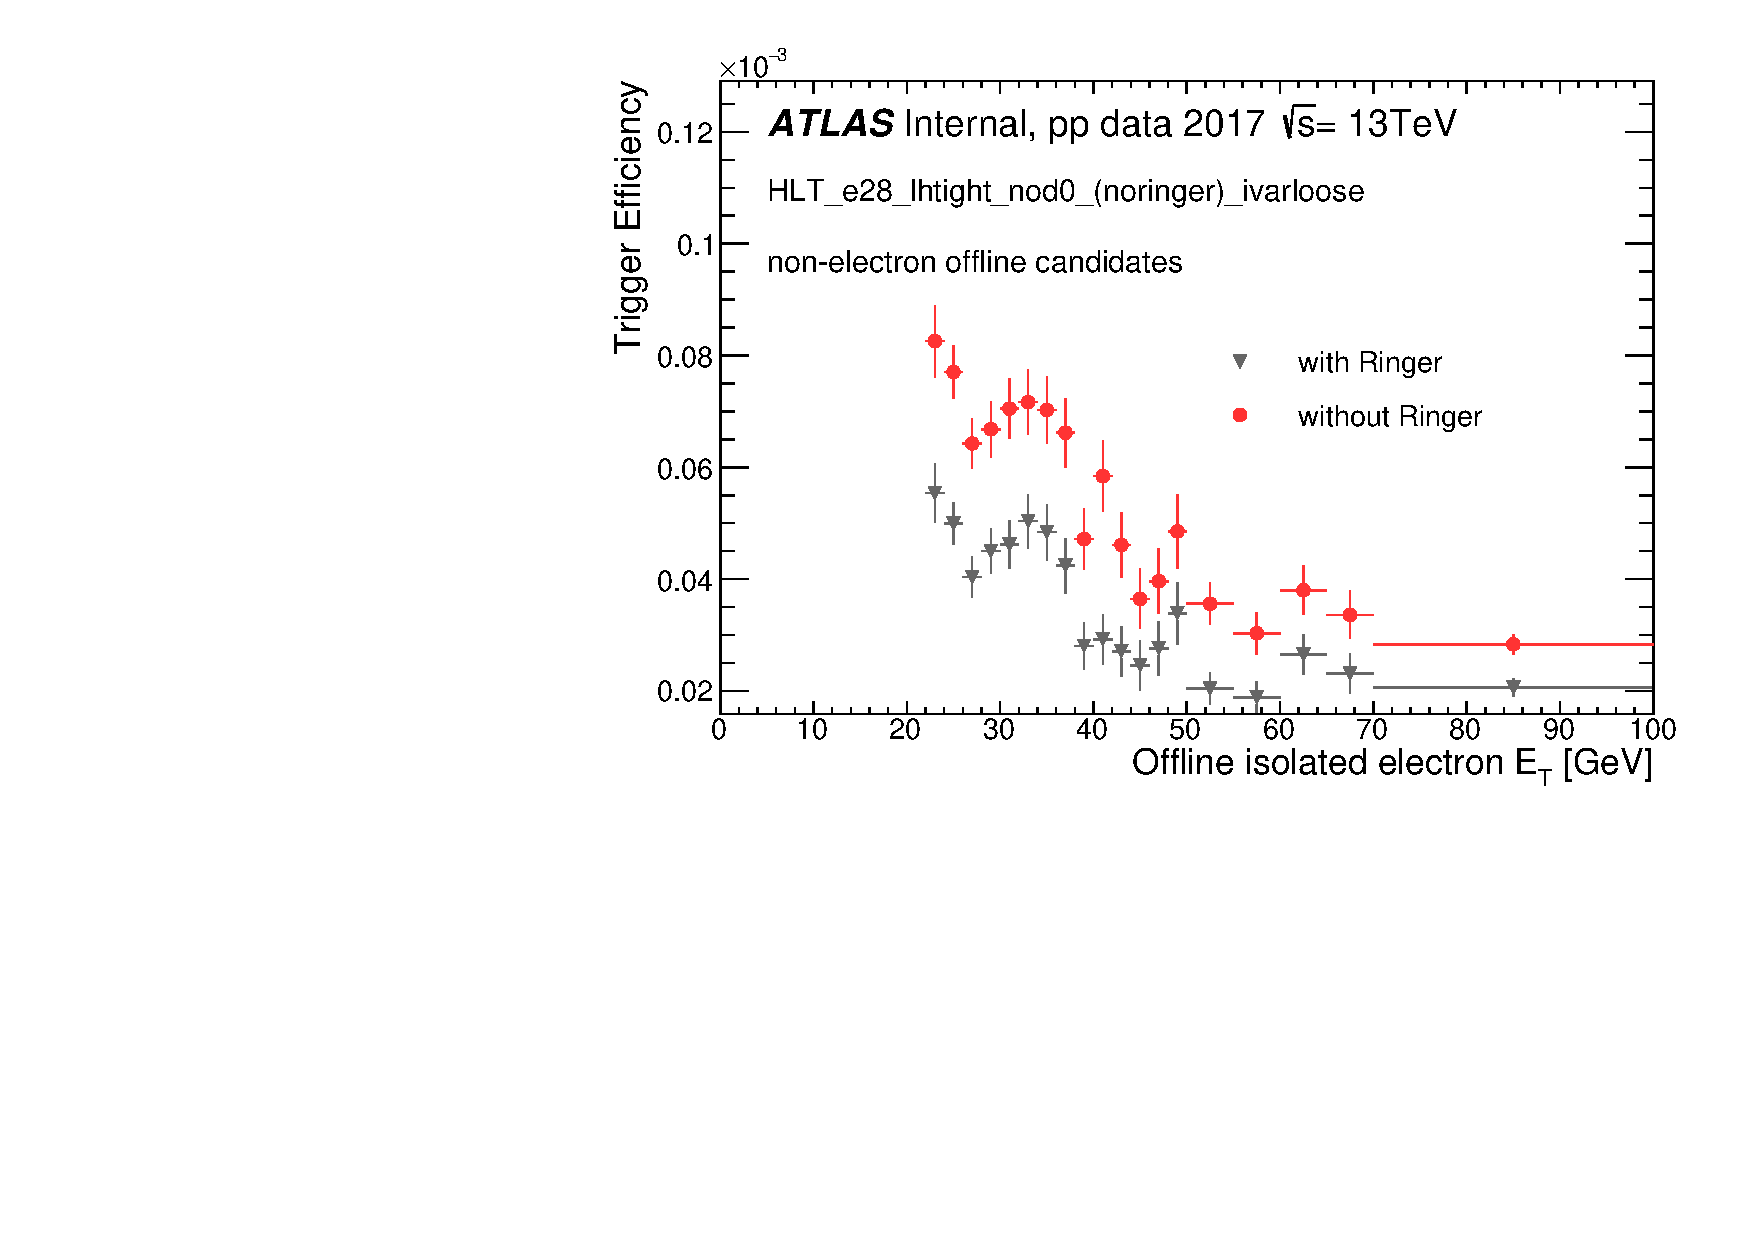
\includegraphics[width=\textwidth]{sections/03_operation/figures/efficiencies/eff_EGAM7_e28_ringer_and_noringer_2017_after_ts1_et.pdf}
  \caption{}
  \end{subfigure}\\
  %
  \begin{subfigure}[c]{.49\textwidth}
  \centering
  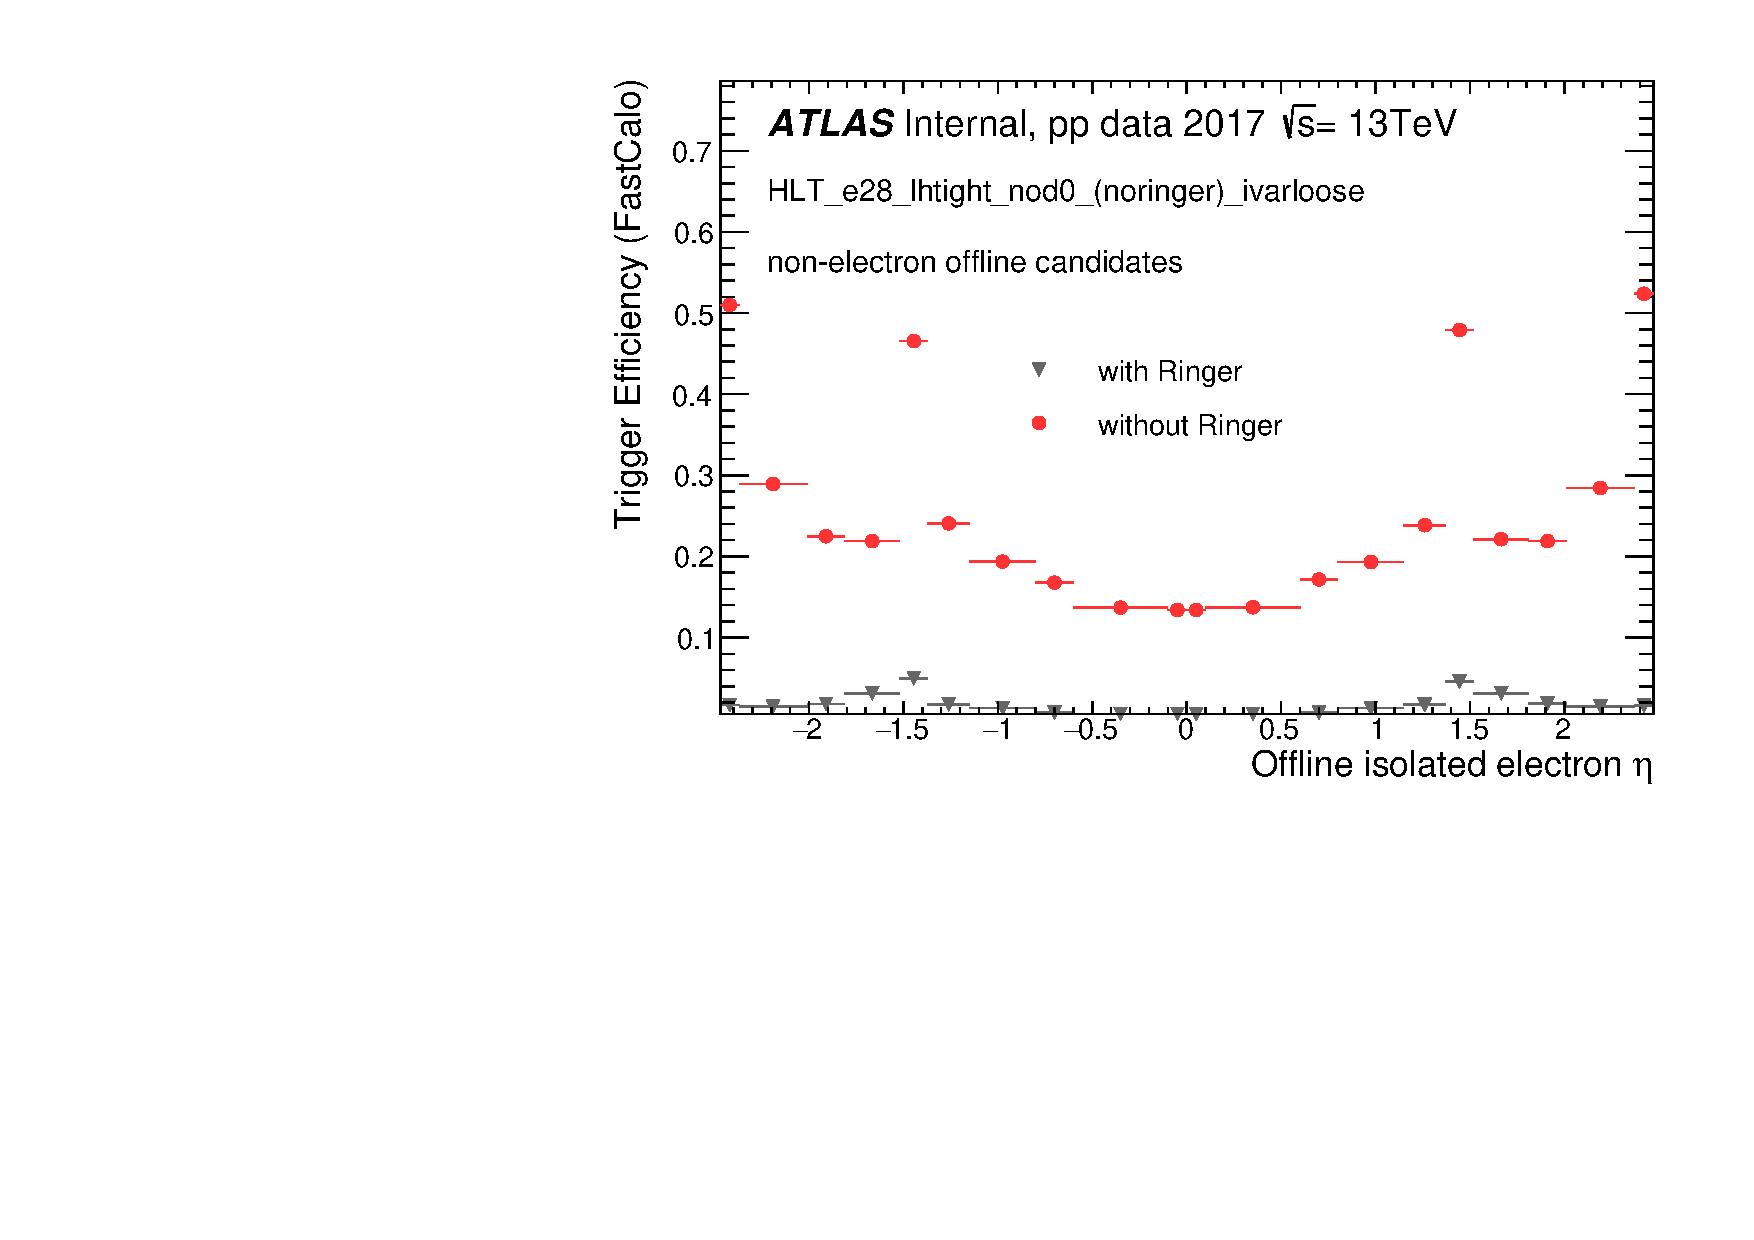
\includegraphics[width=\textwidth]{sections/03_operation/figures/efficiencies/eff_EGAM7_e28_ringer_and_noringer_2017_after_ts1_L2Calo_eta.pdf}
  \caption{}
  \end{subfigure}
  %
  \begin{subfigure}[c]{.49\textwidth}
  \centering
  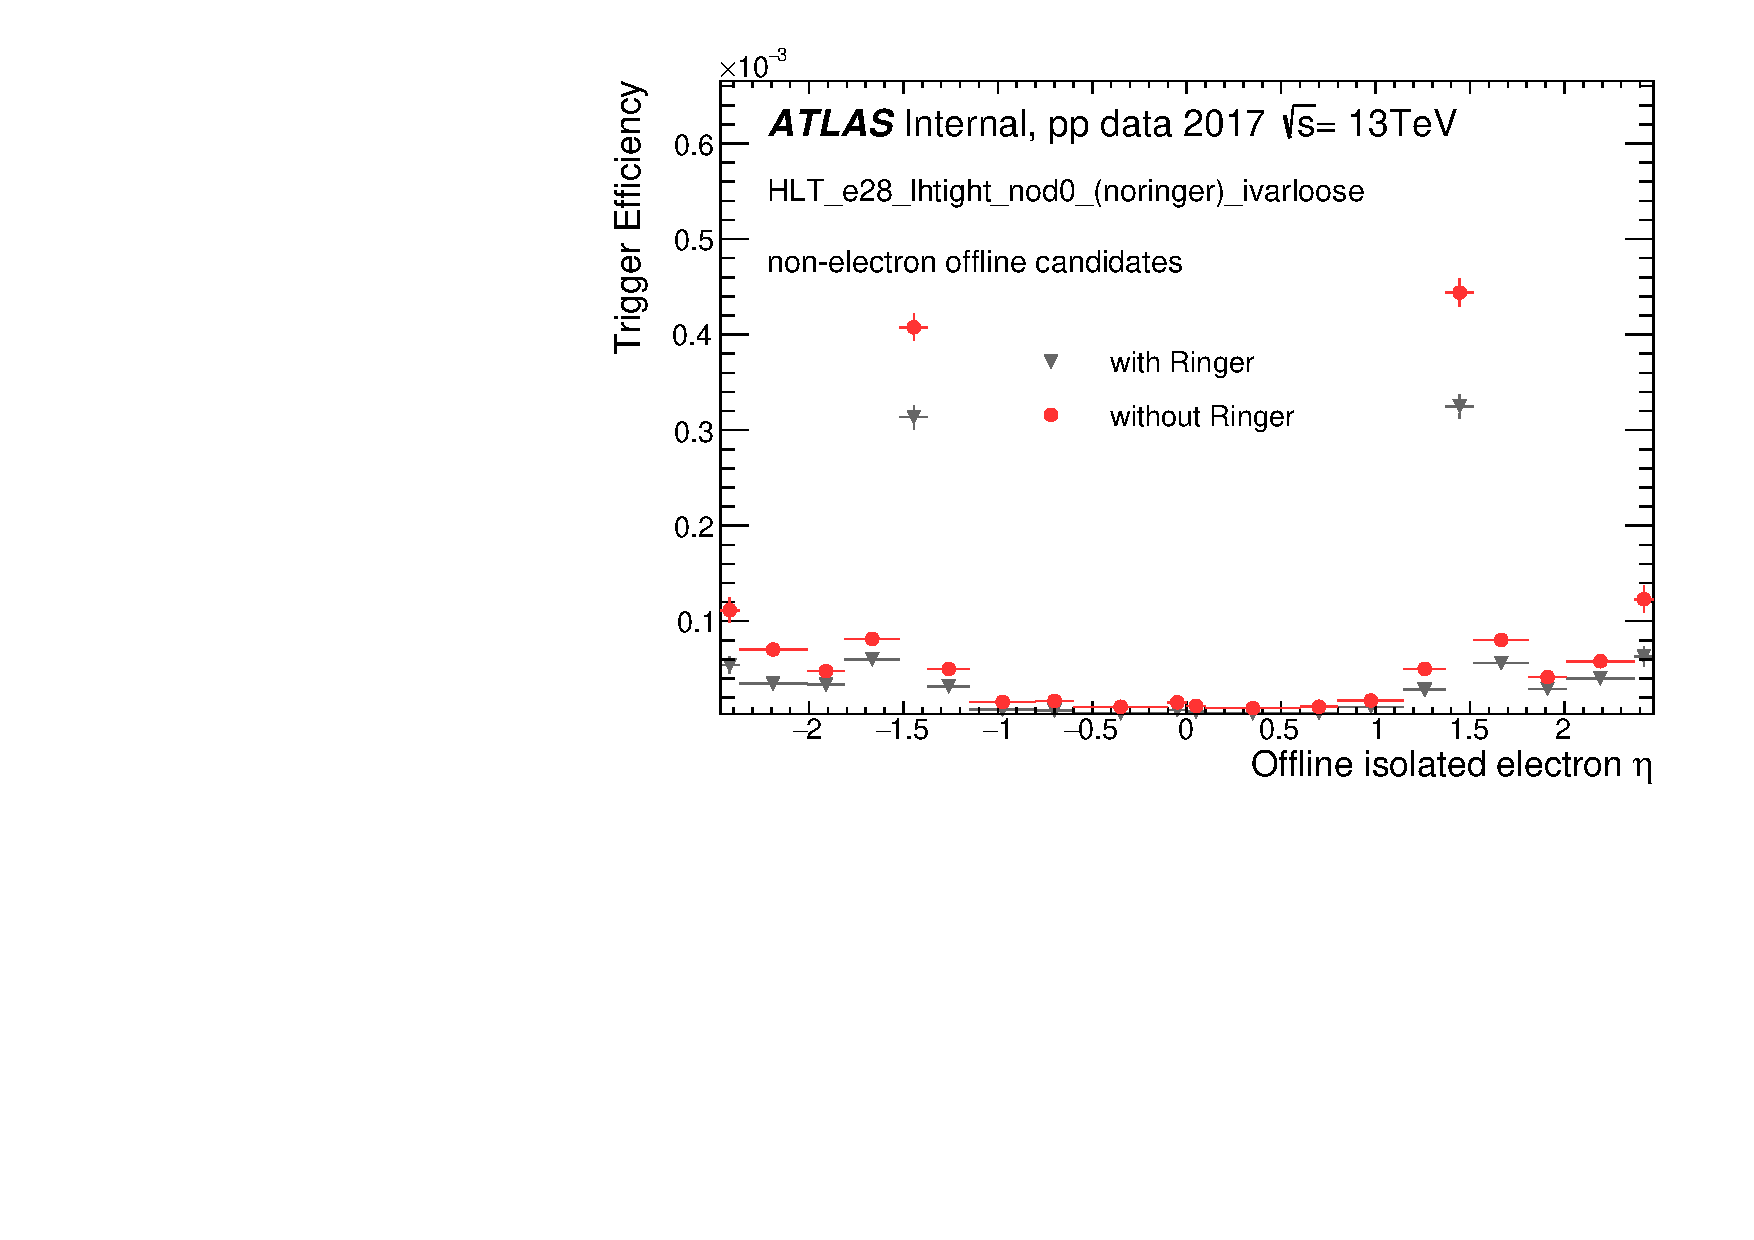
\includegraphics[width=\textwidth]{sections/03_operation/figures/efficiencies/eff_EGAM7_e28_ringer_and_noringer_2017_after_ts1_eta.pdf}
  \caption{}
  \end{subfigure}\\
  %
  \begin{subfigure}[c]{.49\textwidth}
  \centering
  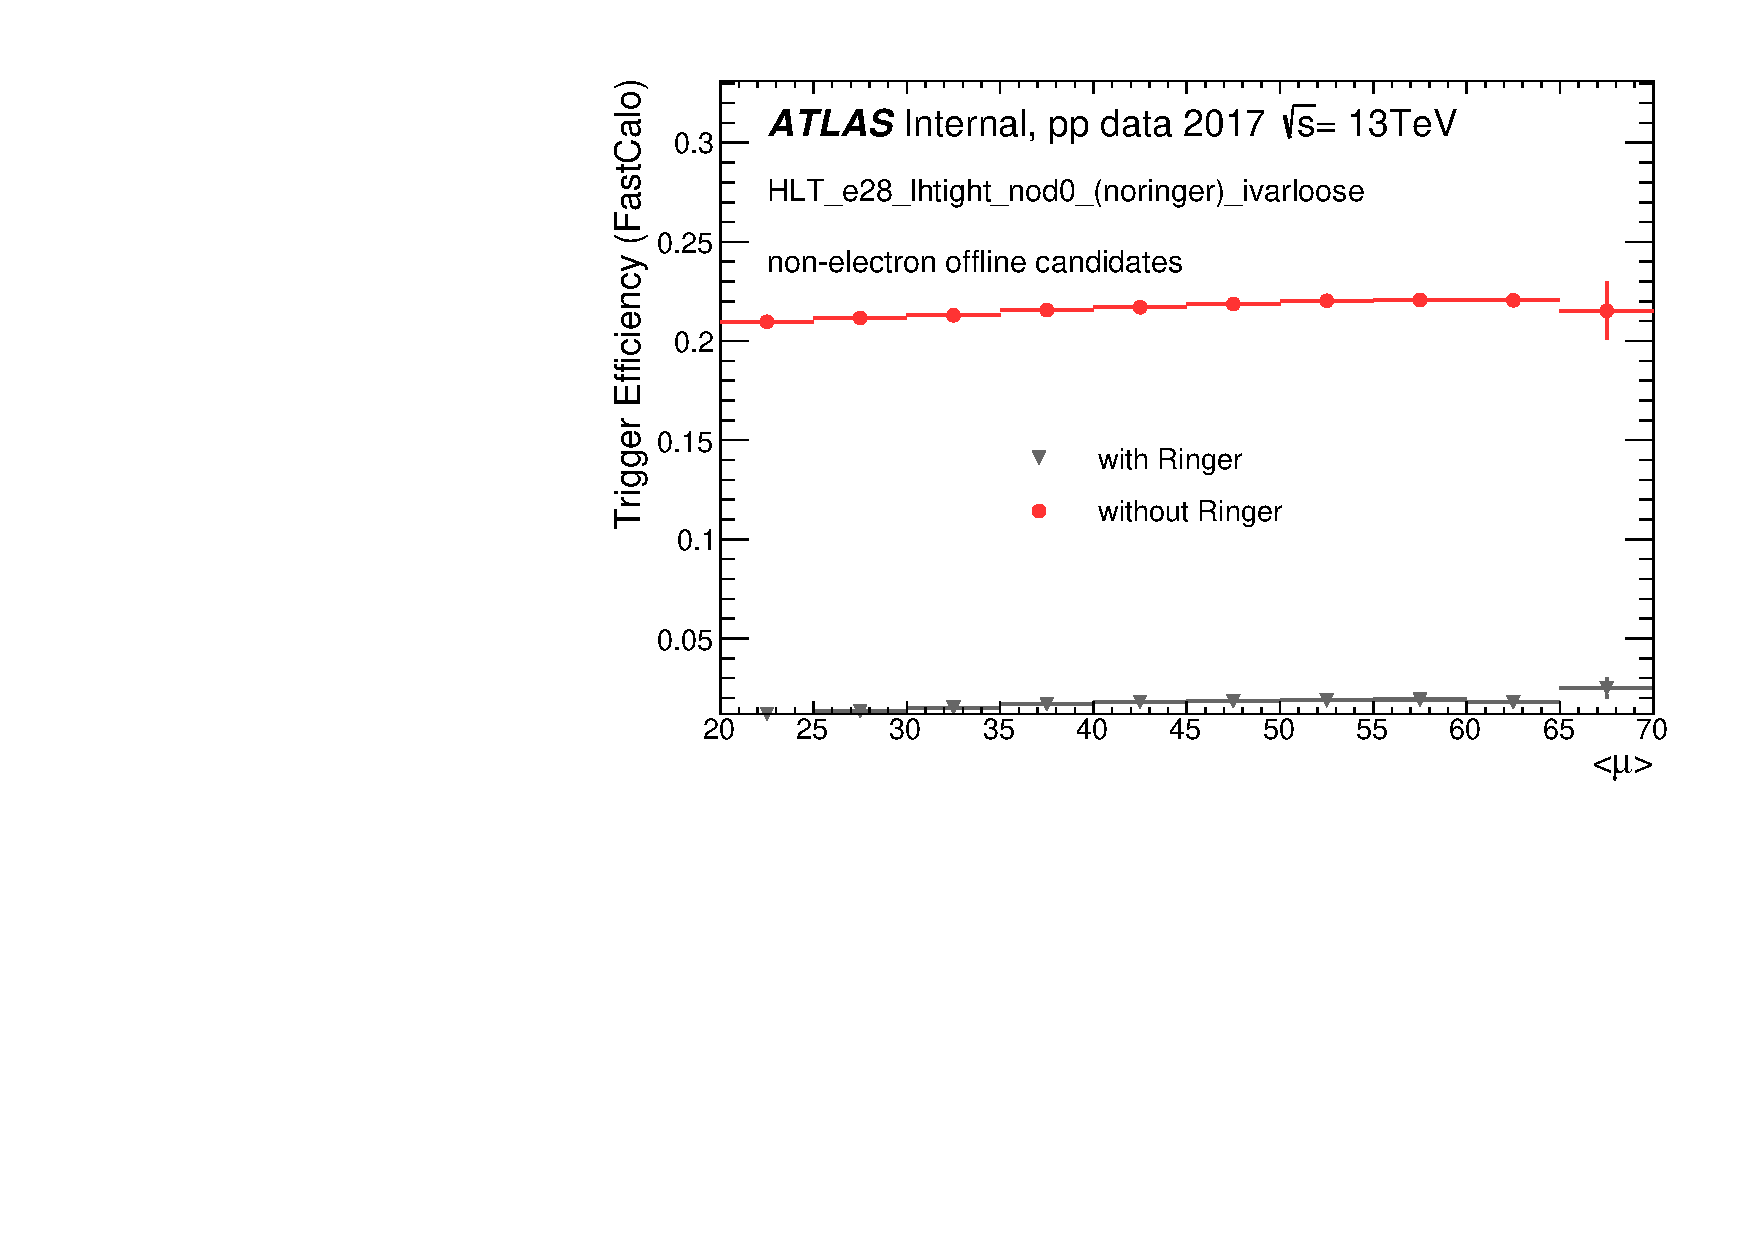
\includegraphics[width=\textwidth]{sections/03_operation/figures/efficiencies/eff_EGAM7_e28_ringer_and_noringer_2017_after_ts1_L2Calo_mu.pdf}
  \caption{}
  \end{subfigure}
  %
  \begin{subfigure}[c]{.49\textwidth}
  \centering
  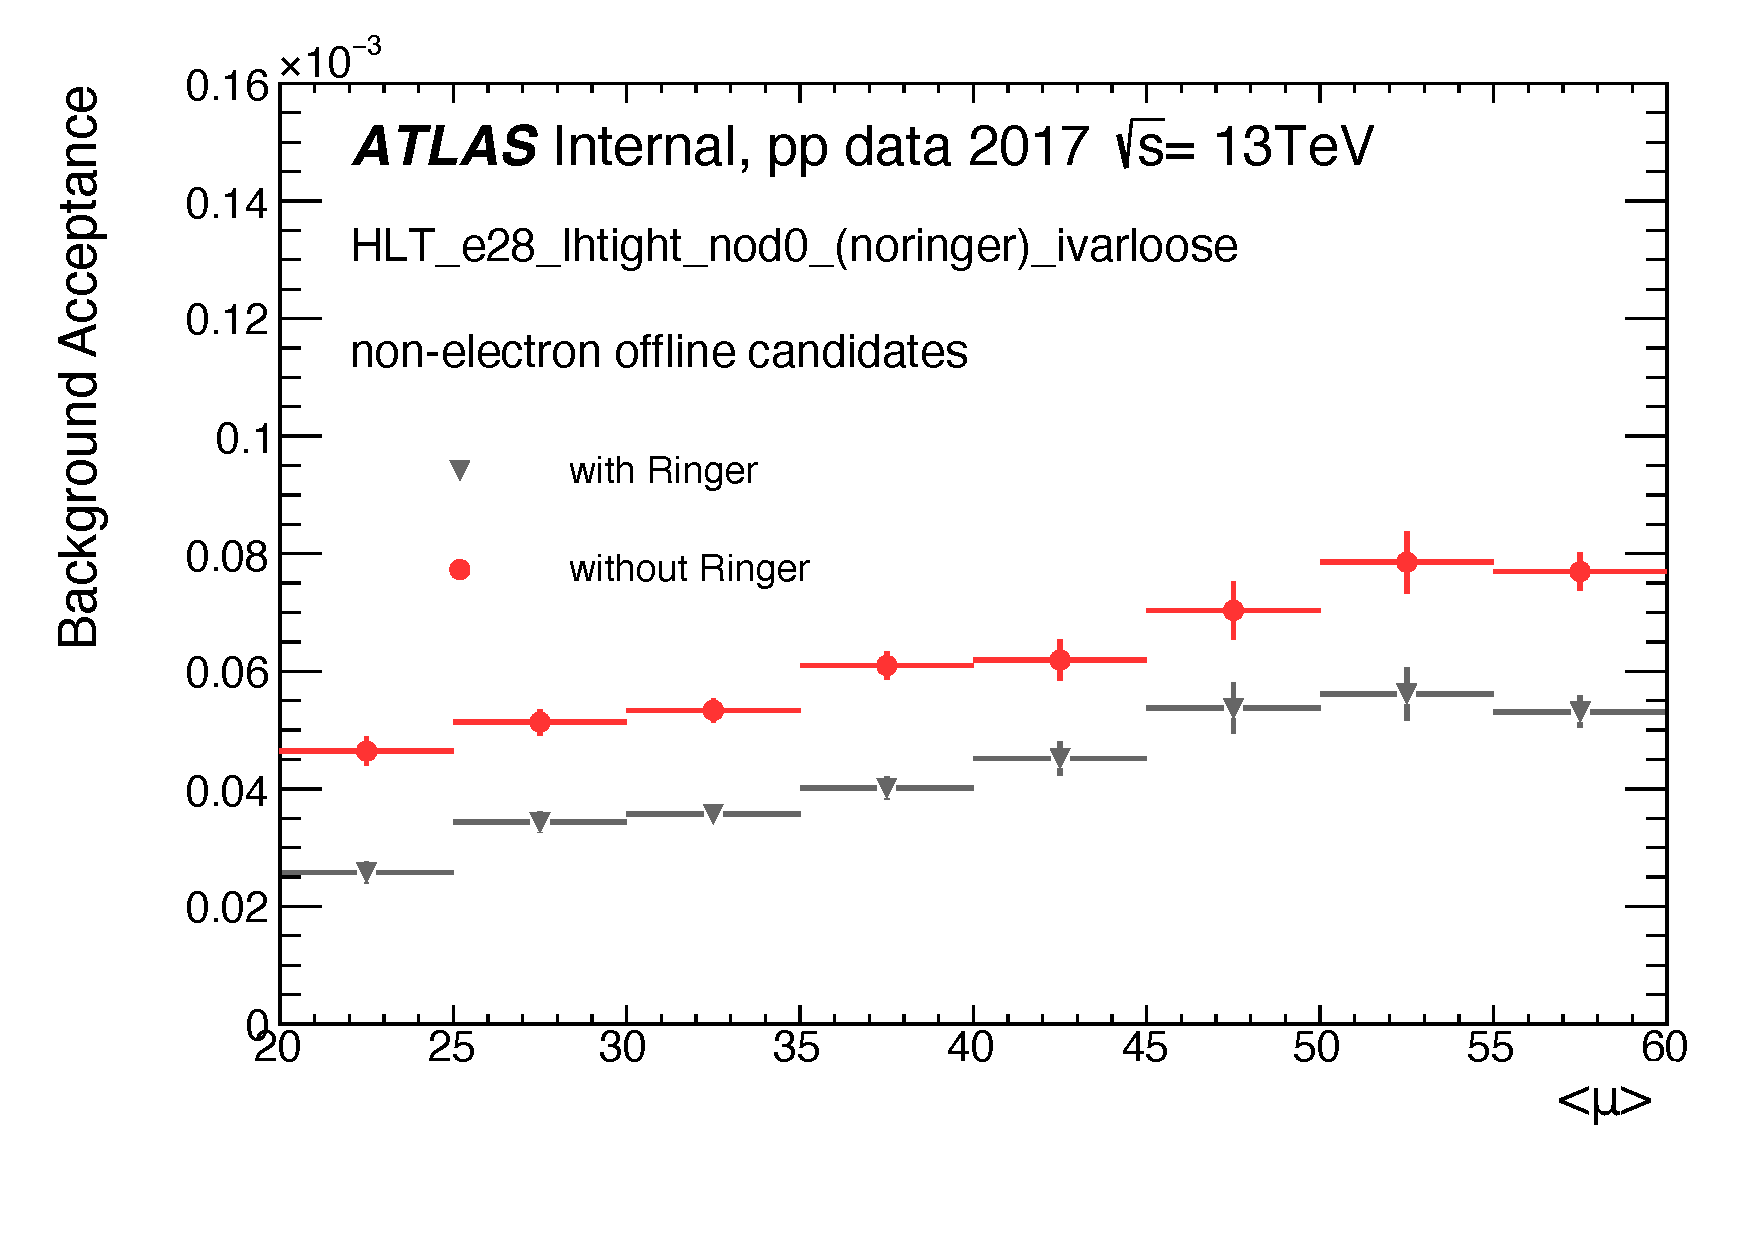
\includegraphics[width=\textwidth]{sections/03_operation/figures/efficiencies/eff_EGAM7_e28_ringer_and_noringer_2017_after_ts1_mu.pdf}
  \caption{}
  \end{subfigure}

  \caption{ Fake electron efficiency as a function for the single electron isolated trigger requiring $\et > \SI{28}{\GeV}$ and \tight selection with and without the \rnn{} algorithm employing 2017 collision data collected after the \rnn algorithm deployment. Left: \fastcalo fake electron efficiency as a function of \et (a), \eta (c) and \avgmu (e). Right: HLT fake electron efficiency as a function of \et (b), \eta (d) and \avgmu (f).}%
  \label{fig:2017_fake_triggers}
\end{figure}




\subsection{2018 Operation}\label{ssec:2018_ringer_operation}

In 2018, the \rnn{} operated with a new tune based on collision data. It was also the case for the final HLT
selection\footnote{One exception was the \medium{} selection, where the HLT likelihood selection operated in 2018 with the same 2017 tune.}. For the lowest-transverse energy-threshold unprescaled trigger, an efficiency improvement of at least one percentage point in central value is observed when comparing both periods, resulting from a better operation in all selection steps, but, in particular, this is due to improvements from the likelihood tunes in the period.

Despite maintaining high electron efficiency, a small reduction in fake acceptance was observed at the  \fastcalo{} step for some unprescaled triggers in comparison with 2017 after TS1. For the lowest-transverse energy-threshold the fake acceptance was reduced by a factor by 1.19. On the other hand, for the highest-transverse energy trigger, a reduction factor by 1.69 was achieved.




\subsection{Impact on CPU Demands} \label{ssec:cpu_reduction}

As observed in the efficiency measurements during 2017-2018 data taking, the \rnn{} allowed for a more effective \fastcalo{} operation in triggers with electrons above \SI{15}{\GeV}  with respect to the previous cut-based approach. 



The overhead required to compute the NN decision by running a single electron trigger with and without the \rnn algorithm, in two individual non-concurrent executions using the same dedicated node\footnote{It was used a techlab node Xeon Phi 7120 (1.7 GHz, 32 threads) with 256 Gb@1333 of memory and a SL6 OS.}, was evaluated. It should be mentioned that, in order to reduce implementation efforts, electron triggers executing the \rnn{} information compute their information after the cut-based reconstruction, whose decision is not computed. As a result of this, the \rnn{} electron triggers always demand additional \fastcalo processing time.

Figures~\ref{fig:fastcalo_fex_time} and~\ref{fig:fastcalo_hypo_time} show the comparison of the total processing time per call for the feature extraction and hypothesis algorithms in the \fastcalo respectively (See the related \fastcalo gray rectangles and diamonds in Figure~\ref{fig:electron_chain}). The processing time per call does not include the online data preparation time. The measurements were evaluated from a very loose selection electron trigger with individual executions in the same dedicated computer node.


The measurement employed events from the enhanced bias (EB)
stream~\cite{eb_description} typically extracted from one hour acquisition with
a specific trigger menu based only on first level selection and aiming at
collecting about one million background events more likely to be accepted by the
\hlt{}. This behavior is obtained by applying an increased weighting in high-\pt{} region,
and at a output trigger rate of \SI{300}{\hertz}~\cite{eb_specifications} for one hour. Hence, the measurements are performed under pile-up conditions with the execution of the
reconstructed observable algorithm for multiple RoIs in the same bunch-crossing event.


\begin{figure}[h!tb]
	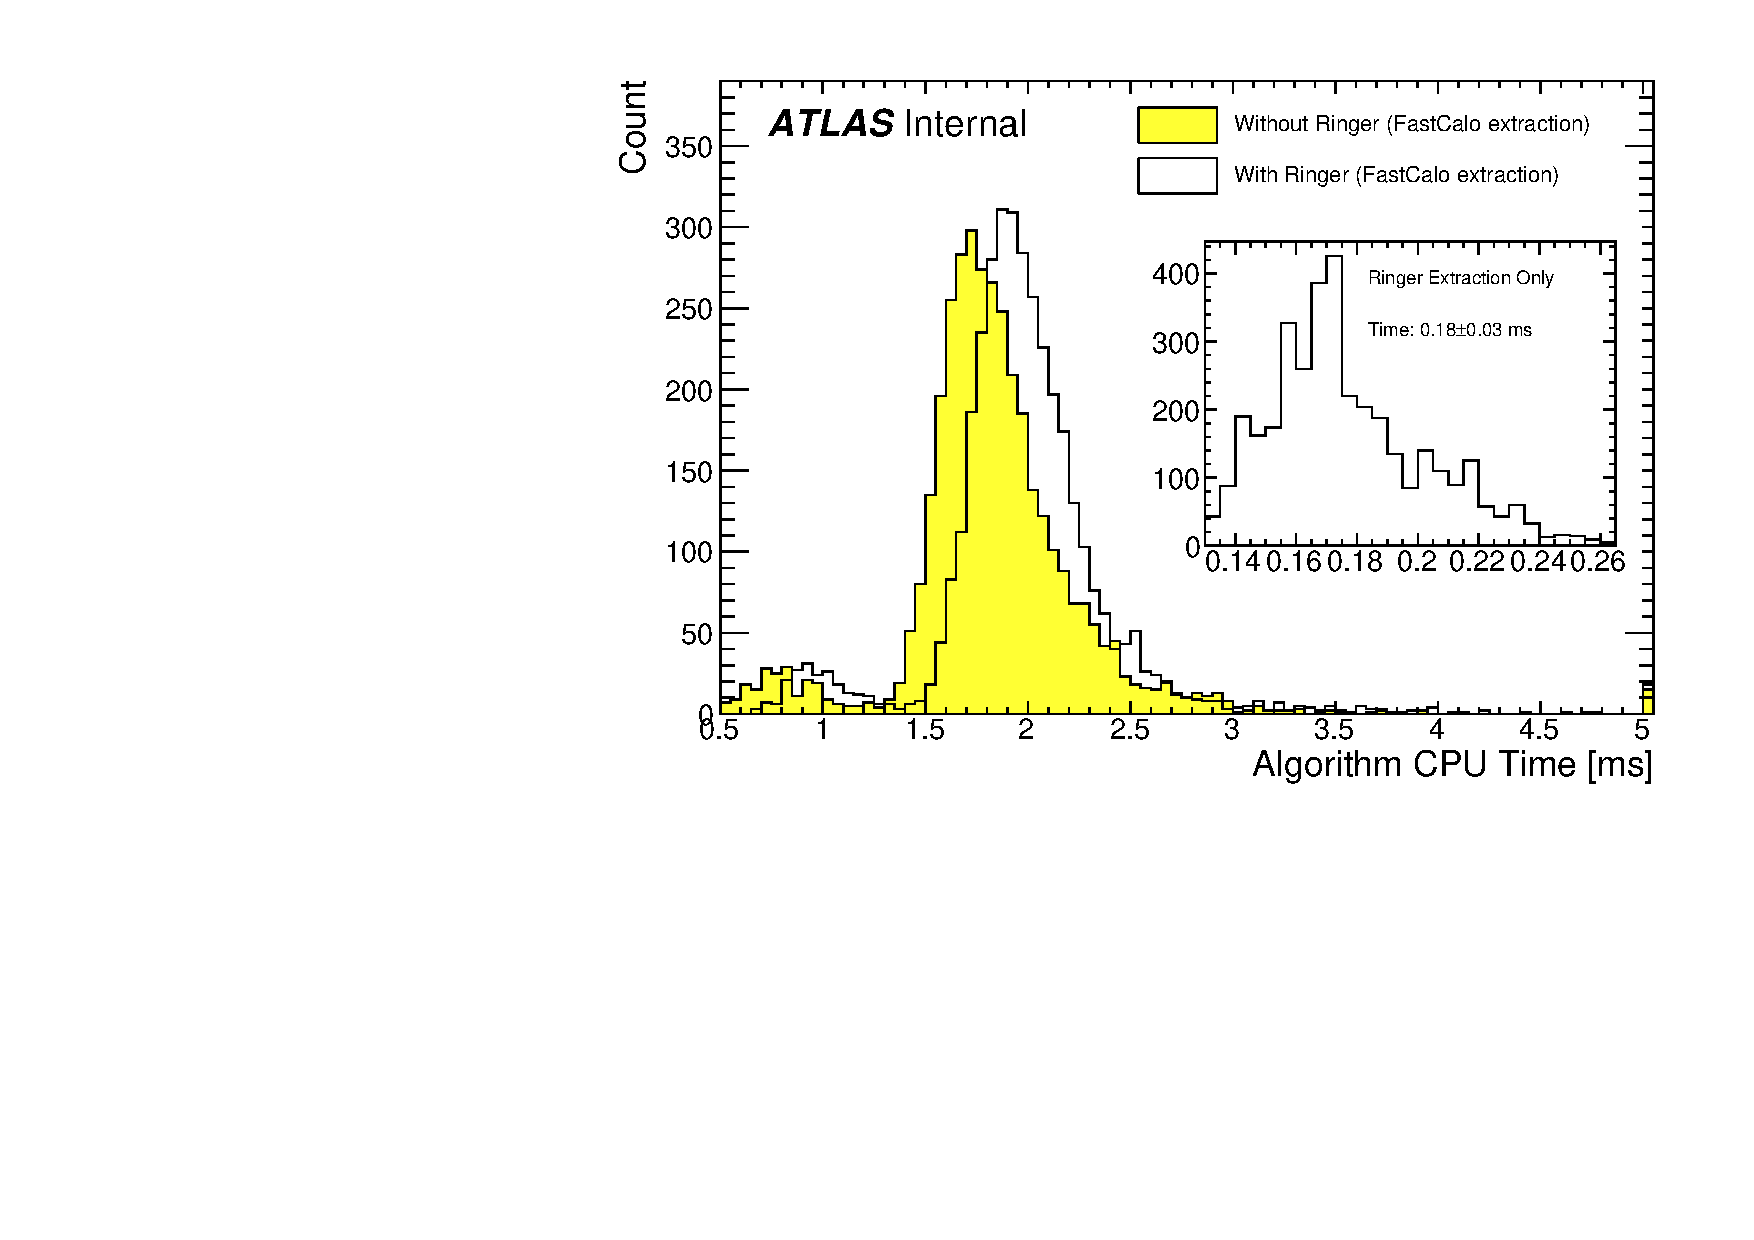
\includegraphics[width=.7\textwidth]{sections/03_operation/figures/EgammaFex_TotalTime}
	\centering
	\caption{\label{fig:fastcalo_fex_time}
		Total processing time per call for the feature extraction algorithms in the \fastcalo step of electron offline rerunning triggers with (white) and without (yellow) \rnn{} using EB events ($\avgmu=45$ peak). Detail on the right shows the individual processing time per call of the ring variable extraction.  
	}
\end{figure}

\begin{figure}[h!tb]
	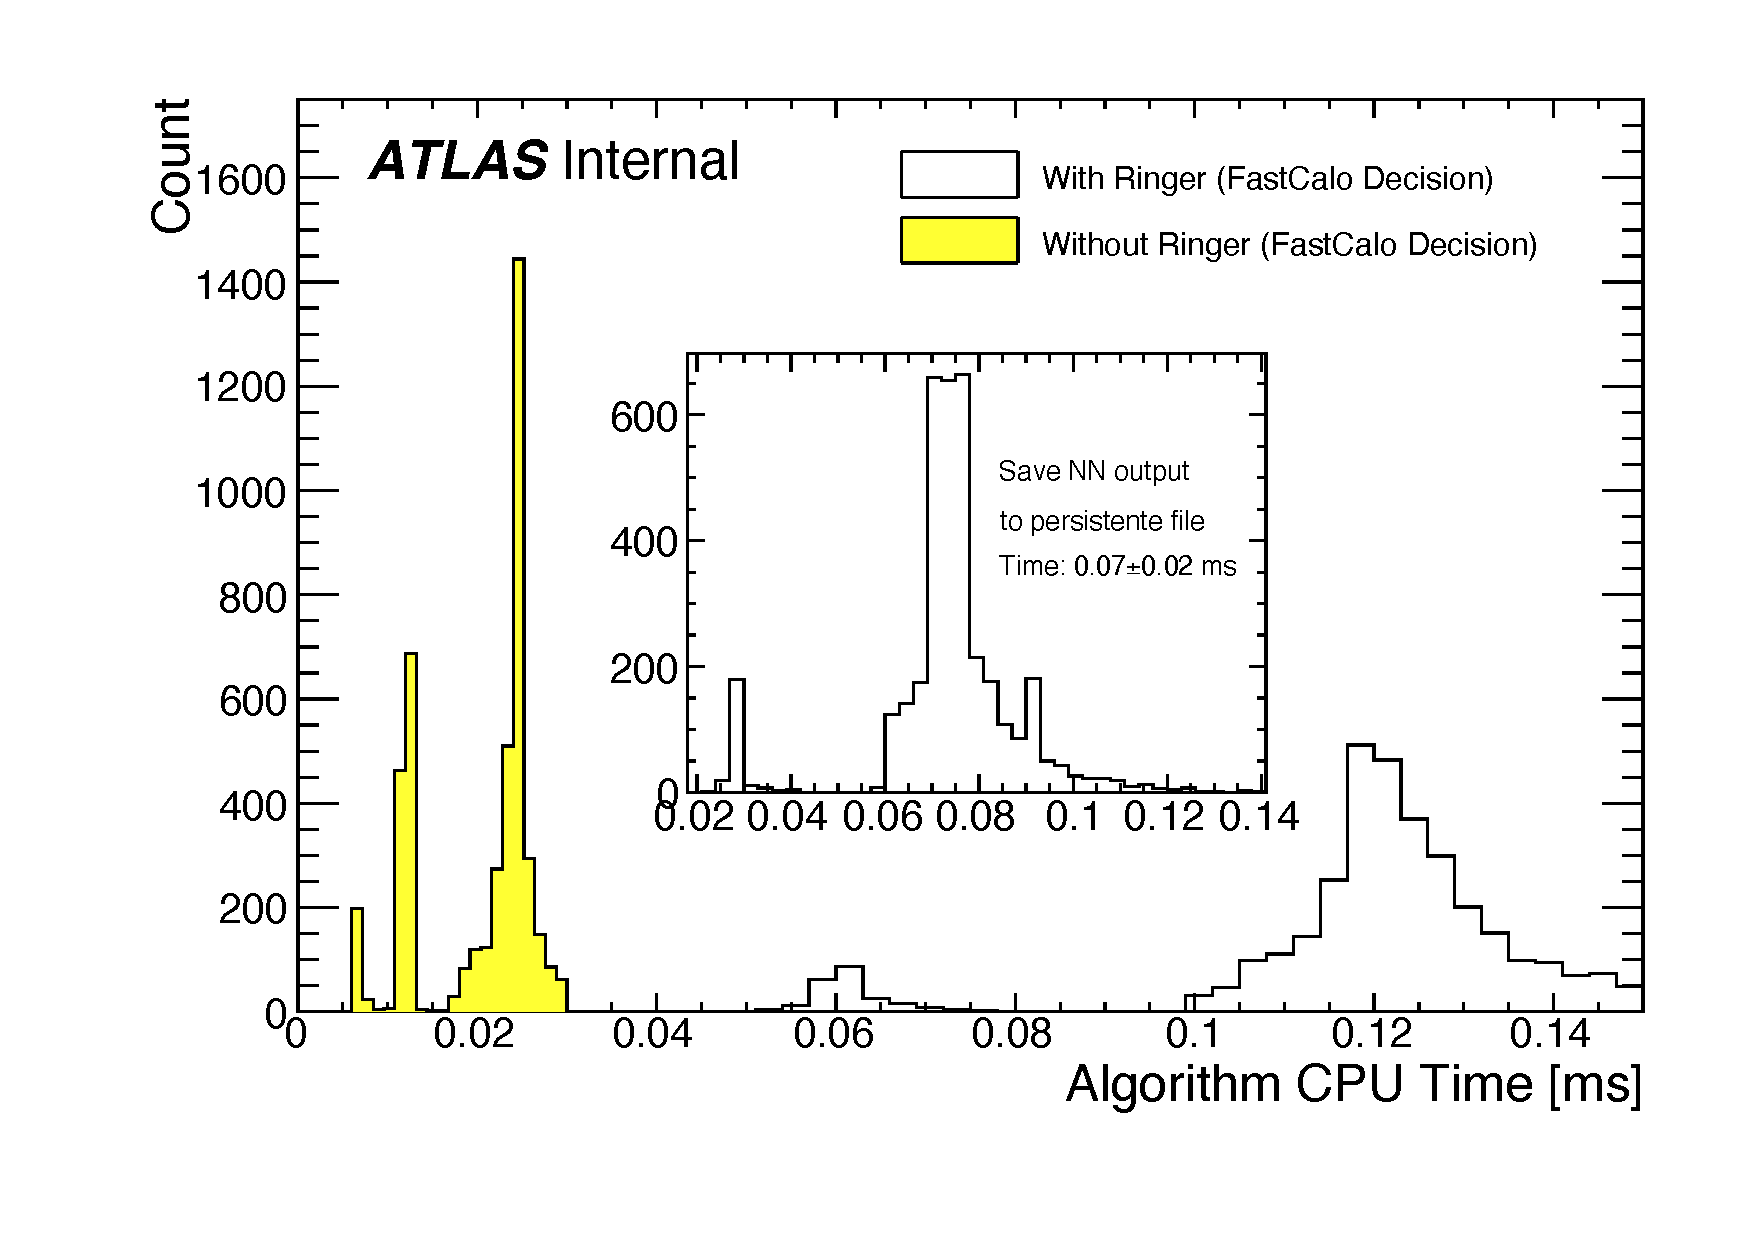
\includegraphics[width=.7\textwidth]{sections/03_operation/figures/EgammaHypo_TotalTime.pdf}
	\centering
	\caption{\label{fig:fastcalo_hypo_time}
		Total processing time per call for the hypothesis testing algorithms
		in the \fastcalo step of electron offline rerunning triggers with (white) and without (yellow) \rnn{} using EB events ($\langle \mu \rangle = 45$ peak). The center histogram represents the individual processing time per call to store the \rnn{} output in persistent file format.}
\end{figure}

A multi-modal structure can be observed in the feature extraction distributions of both trigger configurations, which is associated to the algorithm for retrieving the EM2 cells and building related shower shape
variables\footnote{The three peak structure comes from the raw data conversion. Particularly, these are amongst the most-demanding contributions to the \fastcalo total CPU time.}. The computation of the ring variables, the only difference between the triggers in the \fastcalo feature extraction, requires an additional average processing time of \SI{0.18 \pm 0.03}{\ms/\text{event}}. 


A less relevant contribution comes from hypothesis testing, in which the ring variables are normalized, the discriminating is computed, compared to the selection requirement and stored into the persistent file format\footnote{For Run-3 this step has been removed as a way to reduce the CPU time at \fastcalo step.}. Specifically, \rnn{} hypothesis testing is considerably more demanding, up to \SI{0.14}{\ms/\text{event}}, mostly due to the time 
to store the neural network output \SI{0.07 \pm 0.02}{\ms/\text{event}}, 
than the cut-based selection (\SI{0.02}{\ms/\text{event}}), however small with respect to the feature extraction values. Additionally, the time increase when compared to the average processing time of a single electron trigger across the entire HLT is still negligible ($\approx 500$ ms in Run 2).

Taking into account the referred values, the \rnn{} can require a
relative increase of up to \SI{50}{\%} in the \fastcalo{} CPU time per event
with respect to the trigger without \rnn{}\footnote{It is expected that the result be dependent on the trigger configuration due to presence of pile-up. Reported results are for e17\_lhvloose\_nod0.}. Nonetheless, the \rnn{} contributes to a more discriminating selection, allowing to reduce CPU demanding triggers by reducing the processing of fake electrons in subsequent steps that are more computationally demanding. In this measurement, where about 3,400 events from the EB stream were considered, the \rnn{} algorithm provided an overall
\SI{60}{\%} reduction (\SI{30.72}{\milli\second} to \SI{10.36}{\milli\second})
in the CPU demands avoiding the computation of fake candidates after the \fastcalo step. 





